\documentclass{standalone}
\usepackage{tikz}
\usetikzlibrary{patterns, positioning}


\begin{document}
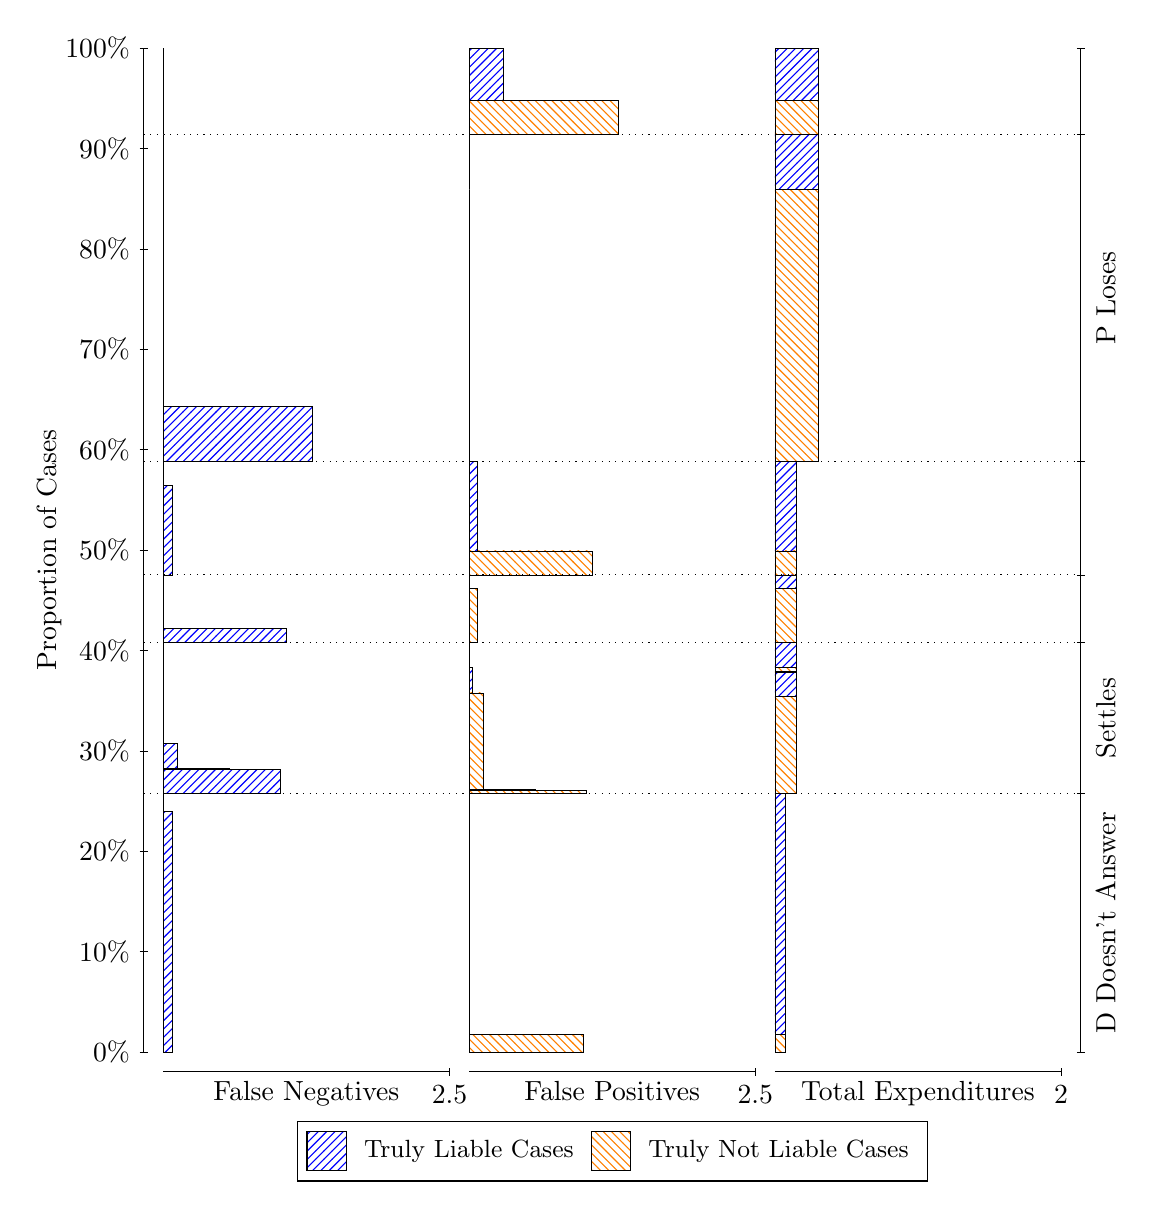
\begin{tikzpicture}
\draw[black, very thin] (1.5,1.75) -- (1.5,14.5);
\node[rotate=90, text=black, anchor=center] at (0.3, 8.125) {Proportion of Cases};
\draw[black, very thin] (1.45,1.75) -- (1.55,1.75);
\node[text=black, anchor=east] at (1.45, 1.75) {0\%};
\draw[black, very thin] (1.45,3.025) -- (1.55,3.025);
\node[text=black, anchor=east] at (1.45, 3.025) {10\%};
\draw[black, very thin] (1.45,4.3) -- (1.55,4.3);
\node[text=black, anchor=east] at (1.45, 4.3) {20\%};
\draw[black, very thin] (1.45,5.575) -- (1.55,5.575);
\node[text=black, anchor=east] at (1.45, 5.575) {30\%};
\draw[black, very thin] (1.45,6.85) -- (1.55,6.85);
\node[text=black, anchor=east] at (1.45, 6.85) {40\%};
\draw[black, very thin] (1.45,8.125) -- (1.55,8.125);
\node[text=black, anchor=east] at (1.45, 8.125) {50\%};
\draw[black, very thin] (1.45,9.4) -- (1.55,9.4);
\node[text=black, anchor=east] at (1.45, 9.4) {60\%};
\draw[black, very thin] (1.45,10.675) -- (1.55,10.675);
\node[text=black, anchor=east] at (1.45, 10.675) {70\%};
\draw[black, very thin] (1.45,11.95) -- (1.55,11.95);
\node[text=black, anchor=east] at (1.45, 11.95) {80\%};
\draw[black, very thin] (1.45,13.225) -- (1.55,13.225);
\node[text=black, anchor=east] at (1.45, 13.225) {90\%};
\draw[black, very thin] (1.45,14.5) -- (1.55,14.5);
\node[text=black, anchor=east] at (1.45, 14.5) {100\%};

\draw[black, very thin] (13.4,1.75) -- (13.4,14.5);
\draw[black, very thin] (13.35,1.75) -- (13.45,1.75);
\node[anchor=west] at (13.35, 1.75) {};
\draw[black, very thin] (13.35,5.03) -- (13.45,5.03);
\node[anchor=west] at (13.35, 5.03) {};
\draw[black, very thin] (13.35,6.9538) -- (13.45,6.9538);
\node[anchor=west] at (13.35, 6.9538) {};
\draw[black, very thin] (13.35,7.81) -- (13.45,7.81);
\node[anchor=west] at (13.35, 7.81) {};
\draw[black, very thin] (13.35,9.253) -- (13.45,9.253);
\node[anchor=west] at (13.35, 9.253) {};
\draw[black, very thin] (13.35,13.401) -- (13.45,13.401);
\node[anchor=west] at (13.35, 13.401) {};
\draw[black, very thin] (13.35,14.5) -- (13.45,14.5);
\node[anchor=west] at (13.35, 14.5) {};

\draw[black, very thin, pattern color=blue, pattern=north east lines] (1.75,1.75) rectangle (1.859,4.8091);
\draw[black, very thin, pattern color=orange, pattern=north west lines] (1.75,4.8091) rectangle (1.75,5.03);
\draw[black, very thin, pattern color=blue, pattern=north east lines] (1.75,5.03) rectangle (3.2397,5.335);
\draw[black, very thin, pattern color=blue, pattern=north east lines] (1.75,5.335) rectangle (2.5857,5.353);
\draw[black, very thin, pattern color=blue, pattern=north east lines] (1.75,5.353) rectangle (1.9317,5.672);
\draw[black, very thin, pattern color=orange, pattern=north west lines] (1.75,5.672) rectangle (1.75,6.9538);
\draw[black, very thin, pattern color=blue, pattern=north east lines] (1.75,6.9538) rectangle (3.3123,7.129);
\draw[black, very thin, pattern color=orange, pattern=north west lines] (1.75,7.129) rectangle (1.75,7.81);
\draw[black, very thin, pattern color=blue, pattern=north east lines] (1.75,7.81) rectangle (1.859,8.9499);
\draw[black, very thin, pattern color=orange, pattern=north west lines] (1.75,8.9499) rectangle (1.75,9.253);
\draw[black, very thin, pattern color=blue, pattern=north east lines] (1.75,9.253) rectangle (3.6393,9.9504);
\draw[black, very thin, pattern color=orange, pattern=north west lines] (1.75,9.9504) rectangle (1.75,13.401);
\draw[black, very thin, pattern color=orange, pattern=north west lines] (1.75,13.401) rectangle (1.75,13.839);
\draw[black, very thin, pattern color=blue, pattern=north east lines] (1.75,13.839) rectangle (1.75,14.5);
\draw[black, very thin, pattern color=orange, pattern=north west lines] (5.6333,1.75) rectangle (7.0867,1.9708);
\draw[black, very thin, pattern color=blue, pattern=north east lines] (5.6333,1.9708) rectangle (5.6333,5.03);
\draw[black, very thin, pattern color=orange, pattern=north west lines] (5.6333,5.03) rectangle (7.123,5.077);
\draw[black, very thin, pattern color=orange, pattern=north west lines] (5.6333,5.077) rectangle (6.469,5.0805);
\draw[black, very thin, pattern color=orange, pattern=north west lines] (5.6333,5.0805) rectangle (5.815,6.3118);
\draw[black, very thin, pattern color=blue, pattern=north east lines] (5.6333,6.3118) rectangle (5.6697,6.6308);
\draw[black, very thin, pattern color=blue, pattern=north east lines] (5.6333,6.6308) rectangle (5.6333,6.9538);
\draw[black, very thin, pattern color=orange, pattern=north west lines] (5.6333,6.9538) rectangle (5.7423,7.6348);
\draw[black, very thin, pattern color=blue, pattern=north east lines] (5.6333,7.6348) rectangle (5.6333,7.81);
\draw[black, very thin, pattern color=orange, pattern=north west lines] (5.6333,7.81) rectangle (7.1957,8.113);
\draw[black, very thin, pattern color=blue, pattern=north east lines] (5.6333,8.113) rectangle (5.7423,9.253);
\draw[black, very thin, pattern color=orange, pattern=north west lines] (5.6333,9.253) rectangle (5.6333,12.704);
\draw[black, very thin, pattern color=blue, pattern=north east lines] (5.6333,12.704) rectangle (5.6333,13.401);
\draw[black, very thin, pattern color=orange, pattern=north west lines] (5.6333,13.401) rectangle (7.5227,13.839);
\draw[black, very thin, pattern color=blue, pattern=north east lines] (5.6333,13.839) rectangle (6.0693,14.5);
\draw[black, very thin, pattern color=orange, pattern=north west lines] (9.5167,1.75) rectangle (9.6529,1.9708);
\draw[black, very thin, pattern color=blue, pattern=north east lines] (9.5167,1.9708) rectangle (9.6529,5.03);
\draw[black, very thin, pattern color=orange, pattern=north west lines] (9.5167,5.03) rectangle (9.7892,6.2613);
\draw[black, very thin, pattern color=blue, pattern=north east lines] (9.5167,6.2613) rectangle (9.7892,6.5662);
\draw[black, very thin, pattern color=orange, pattern=north west lines] (9.5167,6.5662) rectangle (9.7892,6.5697);
\draw[black, very thin, pattern color=blue, pattern=north east lines] (9.5167,6.5697) rectangle (9.7892,6.5878);
\draw[black, very thin, pattern color=orange, pattern=north west lines] (9.5167,6.5878) rectangle (9.7892,6.6348);
\draw[black, very thin, pattern color=blue, pattern=north east lines] (9.5167,6.6348) rectangle (9.7892,6.9538);
\draw[black, very thin, pattern color=orange, pattern=north west lines] (9.5167,6.9538) rectangle (9.7892,7.6348);
\draw[black, very thin, pattern color=blue, pattern=north east lines] (9.5167,7.6348) rectangle (9.7892,7.81);
\draw[black, very thin, pattern color=orange, pattern=north west lines] (9.5167,7.81) rectangle (9.7892,8.113);
\draw[black, very thin, pattern color=blue, pattern=north east lines] (9.5167,8.113) rectangle (9.7892,9.253);
\draw[black, very thin, pattern color=orange, pattern=north west lines] (9.5167,9.253) rectangle (10.062,12.704);
\draw[black, very thin, pattern color=blue, pattern=north east lines] (9.5167,12.704) rectangle (10.062,13.401);
\draw[black, very thin, pattern color=orange, pattern=north west lines] (9.5167,13.401) rectangle (10.062,13.839);
\draw[black, very thin, pattern color=blue, pattern=north east lines] (9.5167,13.839) rectangle (10.062,14.5);
\draw[black, dotted] (1.5,5.03) -- (13.4,5.03);
\draw[black, dotted] (1.5,6.9538) -- (13.4,6.9538);
\draw[black, dotted] (1.5,7.81) -- (13.4,7.81);
\draw[black, dotted] (1.5,9.253) -- (13.4,9.253);
\draw[black, dotted] (1.5,13.401) -- (13.4,13.401);
\draw[black, very thin] (1.75,1.5) -- (5.3833,1.5);
\node[text=black, anchor=north] at (3.5667, 1.5) {False Negatives};
\draw[black, very thin] (5.3833,1.45) -- (5.3833,1.55);
\node[text=black, anchor=north] at (5.3833, 1.45) {2.5};

\draw[black, very thin] (5.6333,1.5) -- (9.2667,1.5);
\node[text=black, anchor=north] at (7.45, 1.5) {False Positives};
\draw[black, very thin] (9.2667,1.45) -- (9.2667,1.55);
\node[text=black, anchor=north] at (9.2667, 1.45) {2.5};

\draw[black, very thin] (9.5167,1.5) -- (13.15,1.5);
\node[text=black, anchor=north] at (11.333, 1.5) {Total Expenditures};
\draw[black, very thin] (13.15,1.45) -- (13.15,1.55);
\node[text=black, anchor=north] at (13.15, 1.45) {2};

\node[text=black, centered, rotate=90] at (13.72, 3.39) {D Doesn't Answer};
\node[text=black, centered, rotate=90] at (13.72, 5.9919) {Settles};


\node[text=black, centered, rotate=90] at (13.72, 11.327) {P Loses};


\draw (7.449999999999999,1.5) node[draw=none] (baseCoordinate) {};
\begin{scope}[align=center]
        \matrix[scale=0.5, draw=black, below=0.5cm of baseCoordinate, nodes={draw}, column sep=0.1cm]{
            \node[rectangle, draw, minimum width=0.5cm, minimum height=0.5cm, pattern color=blue, pattern=north east lines] {}; &
            \node[draw=none, font=\small, text=black] (B) {Truly Liable Cases}; &
            \node[rectangle, draw, minimum width=0.5cm, minimum height=0.5cm, pattern color=orange, pattern=north west lines] {}; &
            \node[draw=none, font=\small, text=black] (B) {Truly Not Liable Cases}; \\
            };
\end{scope}

\end{tikzpicture}
\end{document}